\chapter{Issues with the reward structure}
\begin{quotation}
\noindent ``\emph{quote}''
\begin{flushright}\textbf{author}\end{flushright}
\end{quotation}


\section{Training for more episodes}
If we train for more episodes, only the last one will climb. 

\begin{figure}
	\centering
	\subfloat[][Training over 1 episode]{
		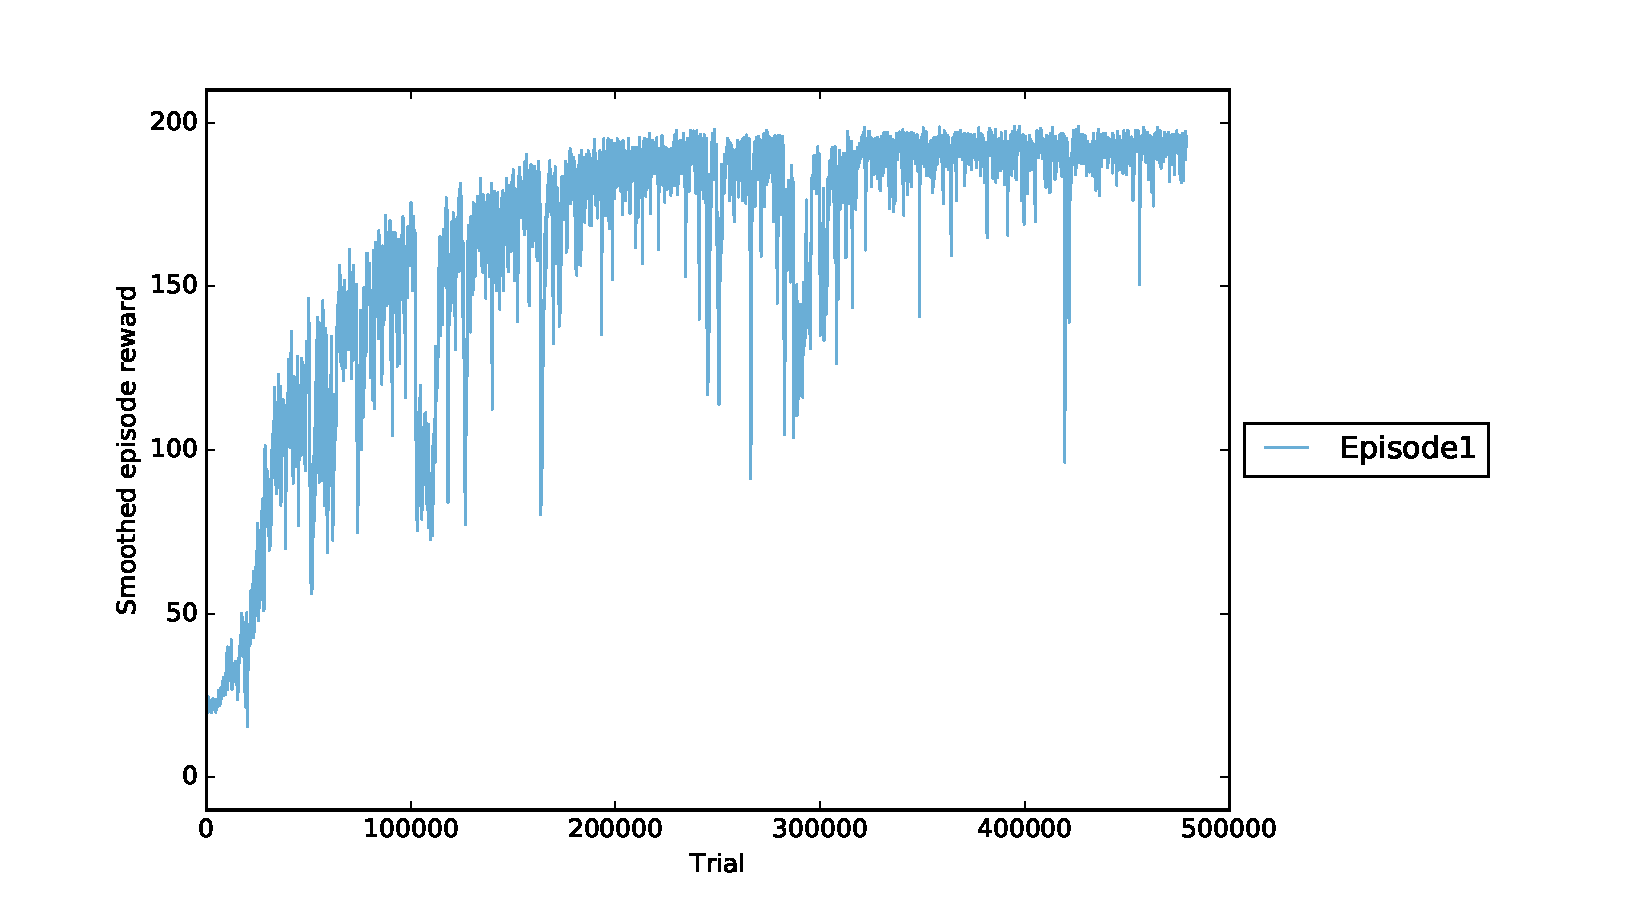
\includegraphics[width=0.49\linewidth]{fig/20permsLR1ep_training.pdf}}
	\subfloat[][Training over 2 episodes]{
		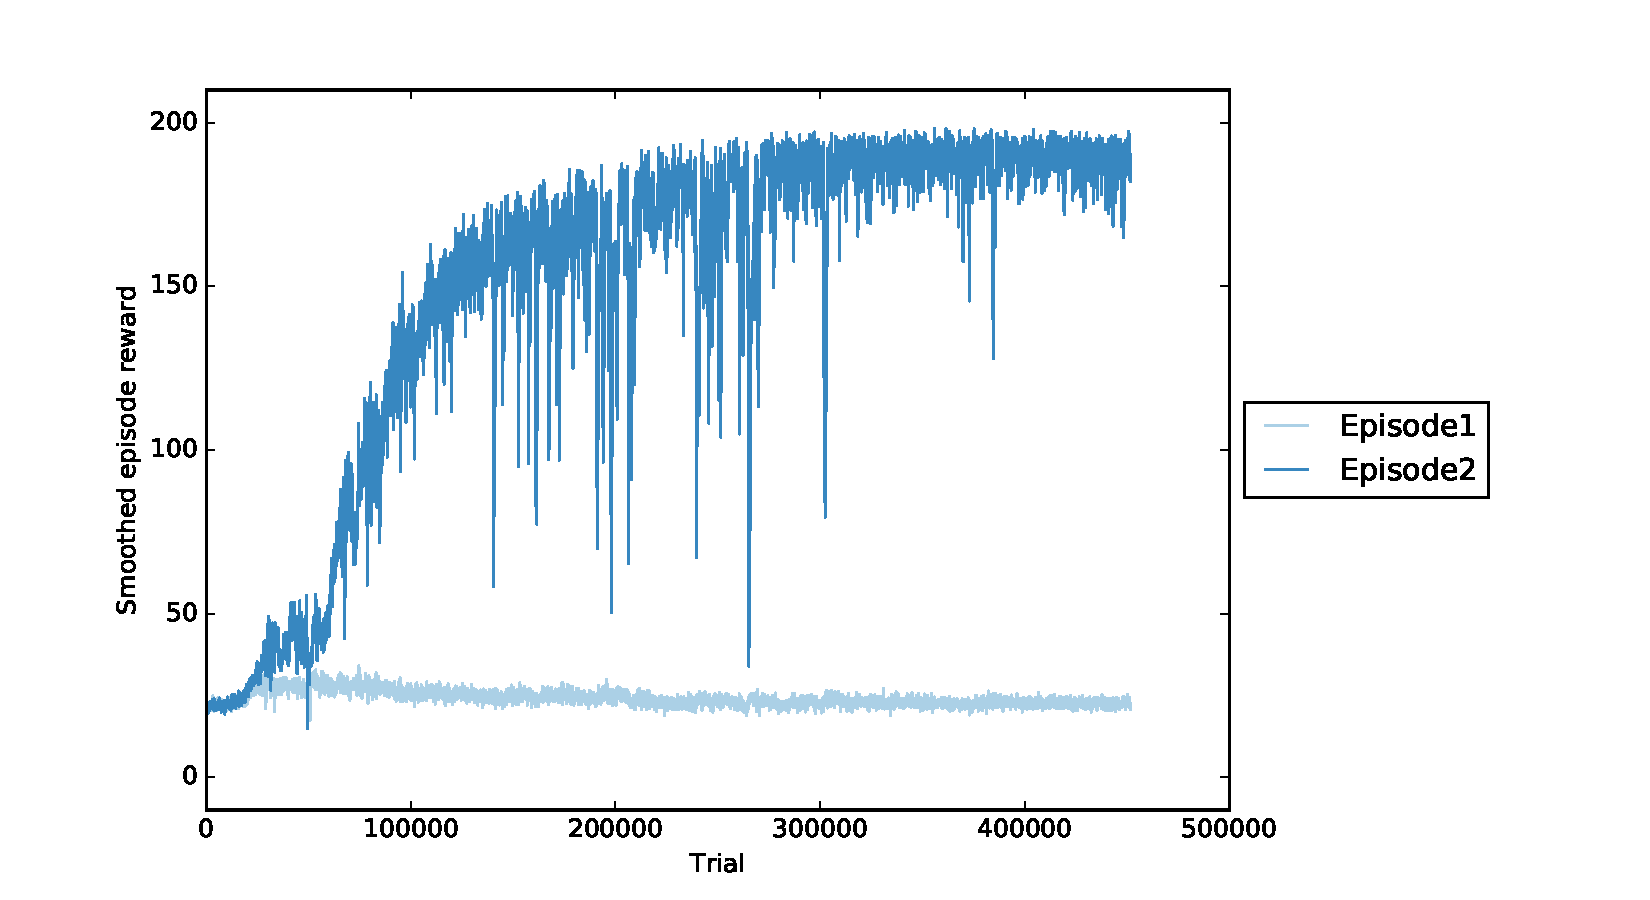
\includegraphics[width=0.49\linewidth]{fig/20permsLR2ep_training.pdf}}
	\\
	\subfloat[][Training over 3 episodes]{
		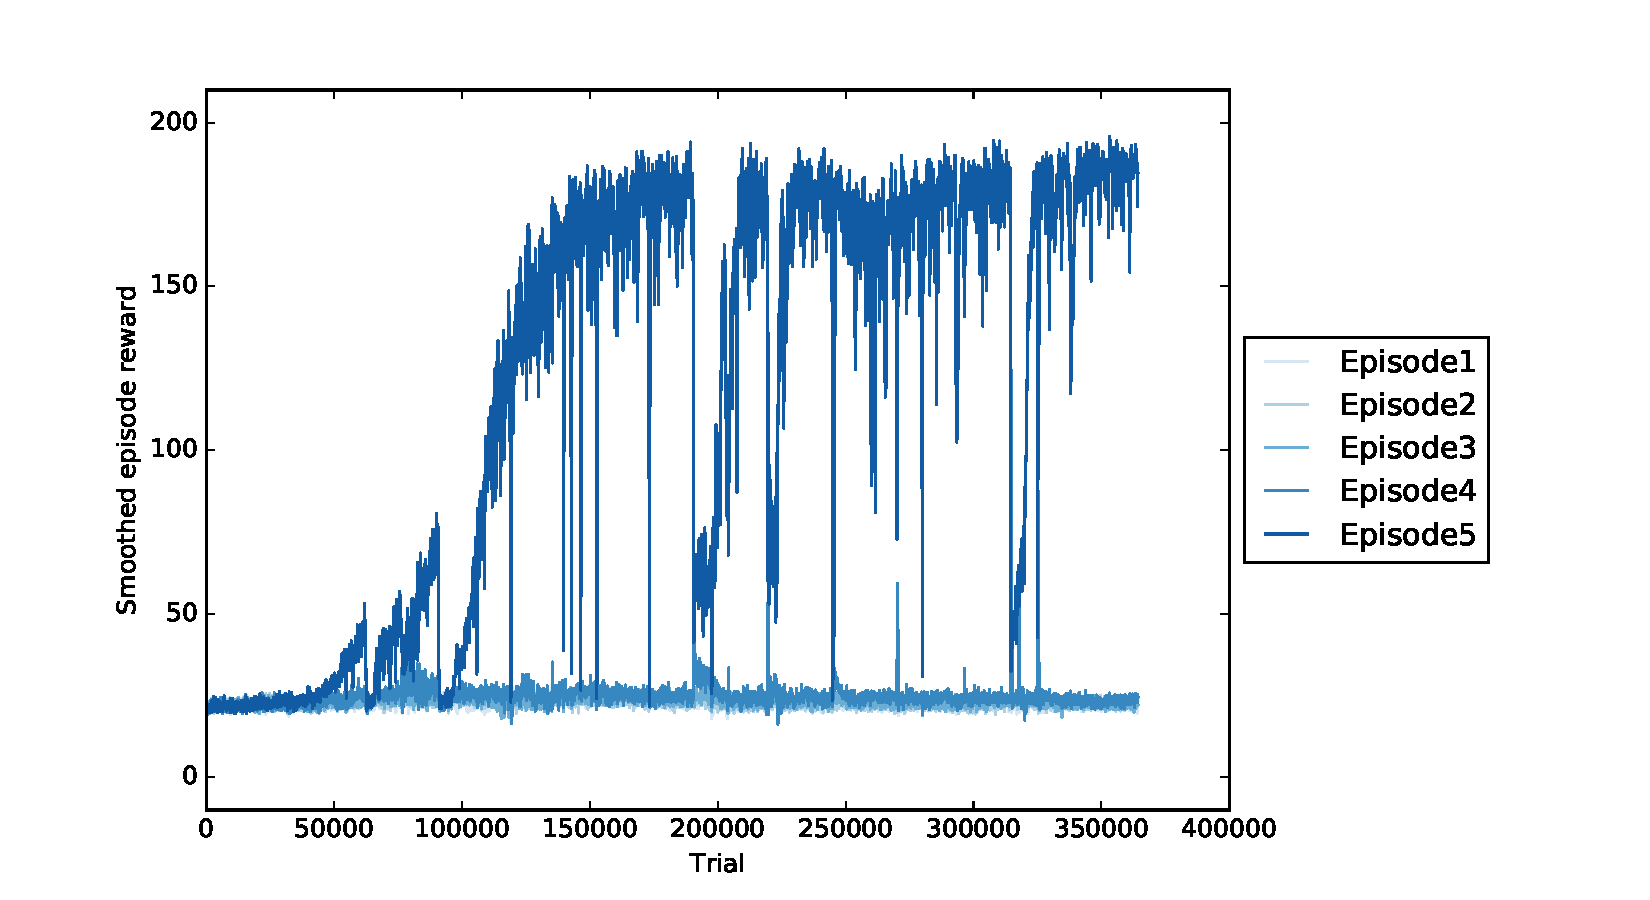
\includegraphics[width=0.9\linewidth]{fig/20permsLR5ep_training.pdf}}
	\caption{}
	\label{fig:20permsLR_training}
\end{figure}

\section{Problems with a 1-per-timestep reward}

\section{Tuning discount factor}
Show different gammas


